\chapter{Related Work}

Multiple authors have already evaluated \acs{DASH} video streaming both in relation to other protocols as seen in \citeauthor{aloman2015performance} but also in a \acs{P2P} network as done by \citeauthor{gazdar2017toward}. In terms of performance of \acs{P2P} networks, \citeauthor{nguyen2009p2p} has evaluated video acquisition with a \acs{DHT} network and \citeauthor{qiu2004modeling} has done a theoretical approach while also listing important aspects to consider when building a \acs{P2P} network. Since the focus of this thesis is on video viewing performance it is also important to consider how videos are watched, which \citeauthor{broxton2013catching} has done by defining a socialness factor to videos, based on how viral they are. Which affects how a video is watched over time in a \acs{P2P} network.

\label{cha:related-work}
\citeauthor{aloman2015performance} \cite{aloman2015performance} have evaluated \acs{DASH} and two other streaming protocols (\acs{RTSP} and \acs{RTMP}) in both on-demand and live in both 4G and Wi-Fi conditions. Evaluation is done in terms of \ac{QOE} metrics with a large amount of parameters including: Resolution, bitrate, framerate, interval between key frames, packet loss rate and delay. \acs{QOE} was estimated through the quality of service through an algorithmic model, rather than user based scores.\\
In terms of results when introduc   tion packet loss and delays \acs{DASH} sacrifices throughput in order to maintain good \acs{QOE} whereas the other instead resort to re-buffering, but \acs{DASH} did have larger initial buffering time, when starting the video, and as packet loss and delay increases more time is required to fill the buffer initially. They conclude that \acs{RTSP} is more efficient for starting the video initially but at the expense of packet loss in the video played stream. They claim this is due to \acs{RTSP} is a UDP based protocol where \acs{DASH} is TCP. But they claim the extra time buffering is worth it as rebuffering events are almost entirely eliminated. In their results \acs{QOE} (measured in MOS) is noticably higher when using \acs{DASH} in the same scenarios. In their testing packet loss affected \acs{QOE} more than delay.

% uses ITU-T Rec P-1201.1\footnote{\url{https://www.itu.int/rec/T-REC-P.1201.1/en}} for non intrusive monitoring of the video.



\citeauthor{gazdar2017toward} \cite{gazdar2017toward} have built a streaming system based on BitTorrent instead of \acs{IPFS}, also using \acs{DASH} as the video format. To accomplish this they needed to make small adjustments to the \acs{MPD} file by adding information about the tracker. This way the \acs{MPD} file alone is enough to start the video streaming process. For tests in the system they focused on segment missing rate and user experience. With a variety of number of peers, start delay and cache sizes. The system got worse performance as the network grew, by having more missed segments and more waiting time on playback. user experience also suffered the most when viewing at a high quality. These conclusions contradict our hypotheses that a large network should help offload the system, but this might be due to BitTorrent not being suitable for this purpose, or that their peer selection algorithm is lacking which they themselves point out might be the case.


\citeauthor{nguyen2009p2p} \cite{nguyen2009p2p} argues that 60\% of the commonly used bandwidth cost can be saved using their \ac{P2P} system as opposed to a client-server model. Their \acs{P2P} uses the \ac{DHT} chord as their network architecture, and the video files are broken into multiple smaller pieces which are then dispersed across peers in the network with redundant copies. To ensure that files are not lost as peers leave and join the network, the new peers share the burden of storing files of the rare pieces, so that it is always possible to reconstruct the video. When streaming a video their system prefers pieces from different peers as this creates multiple internet routes, resulting in higher bit rate. In their testing they store the packets in two ways and compare. The first is to distribute the packets as is (non-\acs{NC}) and the other is having the packets be random linear combinations of the original packets (\ac{RNC}). Their testing results focused on the probability of being able to retrieve a piece and the latency to do so. Where the \acs{RNC} scheme performed best in both.

\citeauthor{qiu2004modeling} \cite{qiu2004modeling} performs a theoretical evaluation of a BitTorrent network, and lists four issues that have to be addressed to understand the system.
Peer evolution is how many peers are in the network and how they are in terms of arrival, departure and bandwidth.
Scalability: The systems performance should increase as number of peers grows, they also state that network performance can be measured by average file downloading time.
File sharing efficiency: The system must be designed such that peers are connected to peers that have the needed file, and the bandwidth of each peer must be fully utilized.
Finally the system needs incentives to prevent free riding, meaning you should not be able to download files without contributing the network.\\
Based on these issues the construct a flow model of a BitTorrent network from which they could infer averages of parameters such as seeds, downloaders and download time as functions of arrival rate. They also proved that BitTorrent had incentives to prevent free riding and a Nash equilibrium existed, meaning the peers would choose their physical upload speed.

\citeauthor{broxton2013catching} \cite{broxton2013catching} have analyzed the characteristics of viral videos on YouTube in terms of how they are viewed in respect to a socialness level they define. They define a social video to be one that is viewed through sharing, meaning that access to the video is done either through an external link, embed of pasting the URL directly. An unsocial video is instead one that is found through a search or some discovery mechanism within the site itself. The socialness level can then be defined by how many of the videos view come from social sources versus nonsocial. The socialness of a video also evolves over time and the percentage of social views drop over time. Meaning the video is shared much more when it is new. They note that highly shared videos tend to generate more views than less shared videos. They also state the socialness of a video varies depending on the genre of the video. The behaviour of social views also depend on the source, social views generated through sites like Twitter drop of harder and peak more in views compared to social views generated through social networks like Facebook.


\section{Frameworks and Technologies}
\label{sec:fram-techn}
In this section frameworks and technologies crucial to or relevant for the thesis are presented.

IPFS figure

\subsection{\acl{IPFS} (\acs{IPFS})}
The \acs{IPFS} is a \acs{P2P} distributed file system, as specified in \cite{benet2014ipfs} and implemented by Protocol Labs\footnote{\url{https://ipfs.io/}}.

It consists of several different properties of successful \acs{P2P} systems such as \acs{DHT}, BitTorrent, Git and \ac{SFS}. The \acs{IPFS} protocol constructed consists of the following sub-protocols, among others;

\subsubsection{Identity}
All nodes are identified by a public key of a SHA-256 cryptographic hash. To instantiate a new identity, the node must solve a static crypto puzzle as utilized in S/Kademlia\cite{baumgart2007skademlia}.

\subsubsection{Routing}
The routing system is capable of finding other peers' addresses in the network and determine which peers serves a wanted object. Using a \acs{DSHT} based on S/Kademlia and Coral \cite{baumgart2007skademlia, freedman2004coral}. A distinction of objects size and use patterns determines where values are stored. If they are less than 1KB they are stored directly on the \acs{DHT}, else a reference of the identity of peers serving the block is stored instead. 

\subsubsection{Exchange}
Distribution of data happens by exchanging blocks with a protocol they call BitSwap, which is inspired by the way BitTorrent exchanges blocks of data. Each peer has a list of blocks they want and a list for which they already have similar to BitTorrent but instead it is for the entire network. In BitSwap value is given to each block, meaning to get something from a another peer something usually has to be given in exchange, if a peer has little or nothing the other peers want it seeks blocks they want prioritized over what is wants itself. Which helps reduce the amount of rare blocks in the network.
The protocol also incentivises seeding even when the peer does not currently need any blocks. The idea is that this debt will be repaid in the future, and as such each peer tracks how much the owe, and they send more blocks to their debtors. The debt is also used as a measure of trusts, which protects versus malicious users.
Nodes also keep ledgers accounting transfers with the other nodes, to track history. When a connection is established Ledger information is exchanged, if it does not match exactly the ledger is recreated from scratch and all accrued trust and debt is reset. The authors claim that malicious users can purposefully lose their debt but is should not be worth the loss in trust.

\subsubsection{Objects}
The individual blocks are linked together using Merkle \acs{DAG}s, which is a directed acyclic graph where the each node has a cryptographic hash, and the hash of the parent verifies the children. This structure is a generalization of the Git data structure and provides. Addressing of content using the hashes, tamper resistance since it can be detected and deduplication as data that holds the same content will also hash to the same thereby only needing to be stored once. From the hash addresses files can also be traversed with a traditional UNIX file system path if the hash is that of a folder.
Since hashes a used to address files, newer versions of a file will hash differently, tracking these is done using additional versioning.


\subsection{\acl{DASH} (\acs{DASH})}

\begin{figure}[bth]
    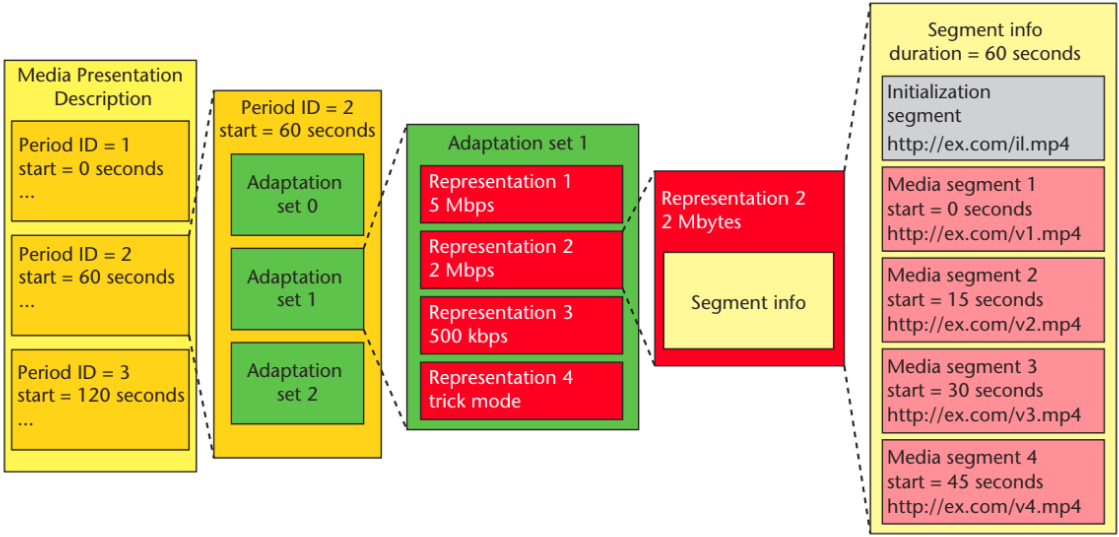
\includegraphics[width=\linewidth]{mpd_structure.png}
    \caption{Structure of the \acs{MPD}.}
    \label{fig:mpd_structure}
    \source{\cite[Figure 3 on p. 65]{sodagar2011mpeg}}
\end{figure}

\ac{DASH} is an adaptive bitrate streaming technique that enables high quality streaming over \acs{HTTP}. This is done by breaking the content into smaller file segments, each containing a short playback interval. Each of these segments are served at different bitrates, allowing the \acs{DASH}-client to choose the next segment to download, based on its current network conditions.
This makes it possible to serve a stream that adapts seamless to deliver streams with high quality and few stalls and re-bufferings, based on the changing conditions of the network.

The segments are described by an \ac{MPD} file, in which information about the files, such as timing, \acs{URL}s, bit rates and resolution resides. From the \acs{MPD} the multimedia selection can then be made based on user preferences (such as specific language audio streams), device capabilities (such as hardware decoding) and the previous mentioned conditions of the network.

The \acs{DASH} Industry Forum (DASH-IF), consisting of Netflix, Google and Microsoft among others, helps push to implementation of the specification\cite{ISO23009}. This is done by creating guidelines for usage and libraries such as \texttt{dash.js}\footnote{\url{https://github.com/Dash-Industry-Forum/dash.js}} that adds \acs{DASH} compatibility in a HTML5 video player using JavaScript.

\subsection{Docker}
Docker\footnote{\url{https://docs.docker.com/}} allows for operating-system-level virtualization, also known as containerization, meaning that the kernel space is shared among instance (containers), but individual user spaces are provided. This makes each container seem like real computers from the point of view of the programs running inside. 
The shared kernel, result in less overhead per container when compared to other virtualization approcahes, but is less flexible since it cannot host a \acs{OS} different from the host machines. Due to the low resource cost of containers, Docker promotes an application-centric container model\cite{merkel2014docker}, so only individual applications or services is run inside, resulting in a loose coupling of the components in the system, as seen with microservices. 

By running programs in containers hardware independence is achieved due to the abstraction layer of Docker, while also gaining easy access to CPU and memory management.

\section{Testing Framework}
\subsection{Chaos Engineering \& Pumba}
\label{sec:framework_pumba}
Chaos Engineering is the discipline of experimenting on a distributed system in order to build confidence in the system’s capability to withstand turbulent conditions in production\footnote{\url{http://principlesofchaos.org/}}.

The philosophy behind Chaos Engineering is that even though each part in a distributed system works correct, systemic weaknesses can exist, and to discover these we emulate and manage chaos inherent in the system. This emperical, systems-based approach builds confidence in the ability of these systems to withstand real conditions, through observations of controlled experiments.

Using Chaos engineering is done by fascillitating an experiment to uncover systemic weakness.
First, a \emph{steady state} is defined by some measureable output, that indicates normal behaviour. The hypothesis is that the \emph{steady state} will continue throughout the experiment.
Secondly, variables that reflect real world events are introduced (eg. server crashes, low bandwidth, spike in traffic, etc.).
Thirdly the hypothesis is tried disproved by examining the \emph{steady state} data.
The harder it is to disrupt a \emph{steady state}, the more confidence is gained in the behaviour of the system, and discovered weaknesses can be targeted for improvement, before the behaviour manifests system-wide.

Netflix developed this practice with their program Chaos Monkey which would randomly shut down services, and later expanded to a set of open sourced tools called Simian Army\footnote{\url{https://github.com/Netflix/SimianArmy}} built for different turbulent conditions, but targeted at \acs{VM}'s.

Pumba\footnote{\url{https://github.com/gaia-adm/pumba}} is a chaos testing tool for containers in Docker. It can manipulate processes, their performance and network.

summary

%%% Local Variables:
%%% mode: latex
%%% TeX-master: "../ClassicThesis"
%%% ispell-dictionary: "british" ***
%%% mode:flyspell ***
%%% mode:auto-fill ***
%%% fill-column: 78 ***
%%% End:
